\begin{center}
    \small ИНФОРМАЦИЯ
\end{center}

\begin{multicols*}{3}

\small \noindent квадрат со стороной 1 так, что на каждой стороне квадрата лежит в точности одна вершина прямоугольника.
\indent 3. Найдите корень уравнения
$$
a x^2+b x+c=0(a \neq 0) .
$$
\noindent если он также является корнем уравнения
$$
b x^2+c x+a=0 .
$$
\noindent 4. Найдите 3 натуральных числа x,y,z, удовлетворяющих уравнению
$$
x^3+y^4=z^7 .
$$
\noindent Докажите, что это уравнение имеет бесконечно много решений в натуральных числах
\normalsize \small Физика
\newline
\indent \small 1. На тело массой M, лежащее на горизонтальной плоскости, начинает действовать переменная сила, направленная под углом $\alpha$ к горизонту(рис.1). Величина силы меняется от 0 до $\infty$. Постройтие график зависимости величины силы трения от величины приложенной сил. Коэффициент трения тела о плоскость $\mu$
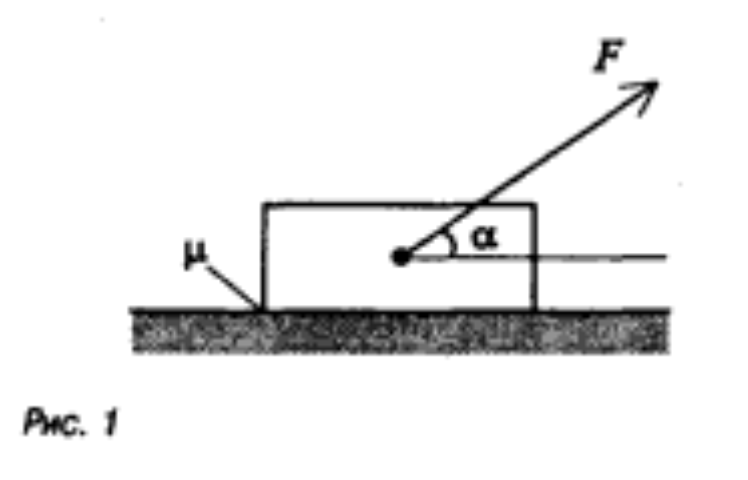
\includegraphics[scale=0.3]{images/image1.png}
\indent \small 2. Два тела, массы которых $m_1$ и $m_2$, связаны пружиной жесткостью $k$ и движутся по гладкому столу под действием силы $F$ (рис.2). Найдите растяжение пружины
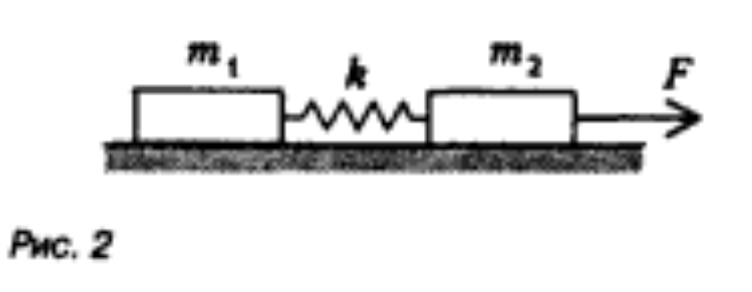
\includegraphics[scale=0.3]{images/image2.png}
\indent \small 3. Тележка массой $M = 4$ кг движется по горизонтальной поверхности со скорость $v_0 = 0,5$ м/с. На тележку вертикально опускают груз массой $m = 1$ кг. Через какой промежуток времени тежелка и груз будут двигаться с одинаковыми скоростями? Коэффициент трения между грузом и тележкой $\mu = 0,1$.
\indent \small 4. Верхний конец лестницы опирается на гладкую стену, а нижний стоит на шероховатом полу. На какое наибольшее расстояние от стены можно отодвинуть нижний конец лестницы, чтобы она не скользила? Длина лестницы $l = 2$ м, коэффициент трения между лестницей и полом $\mu = 0,5$.

\indent \small \textit{10 класс}

\indent \small Математика

\indent \small 1.Найдите положительные (x>0,y>0,z>0) решения системы:
$$
\left\{\begin{array}{l}
\frac{1}{x}+\frac{4}{y}+\frac{9}{z}=3 \\
x+y+z \leq 12
\end{array}\right.
$$
\indent \small 2. Две окружности пересекаются в точках A и B. Отрезок CD проходит через точку A, а отрезок EF - через точку B так, что точки C и E лежат на одной окружности, а точки D и F - на другой, как показано на рисунке 3. Известно, что CE = a, DF=b, а площади четырехугольников ACEB и ADFB равны. Найдите AB.
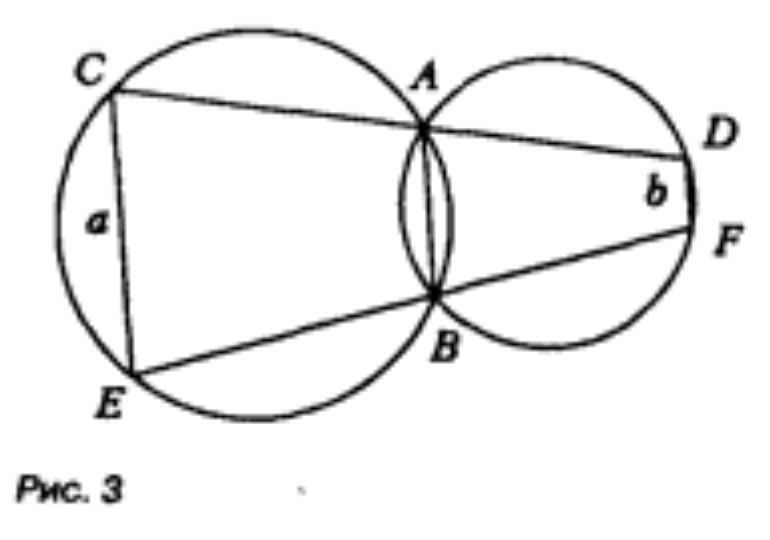
\includegraphics[scale=0.3]{images/image3.png}
\indent \small 3. Уравнения $a x^3+b x^2+c x+d=0$ $(a \neq 0)$ н $b x^3+c x^2+d x+a=0$ нмеют фпий корень. Докажите, что этот корень также удовлетворяет уравнению $c x^3+d x^2+a x+b=0$.

\indent 4. См. задачу 4 для 9 класса.
\indent Физика
\indent 1. Небольшое тело соскальзывает с нулевой начальной скоростью без трения с вершины полусферы радиусовм $R$. На какой высоте тело оторвется от поверхности полусферы?
\indent 2. На горизонтальной поверхности покоится тело, к которому приложена сила $\Vec{F}$(рис. 4). При каких значениях угла $\alpha$ тело будет оставаться в покое независимо от величины силы? Коэффициент трения $\mu$ = = 0,15.
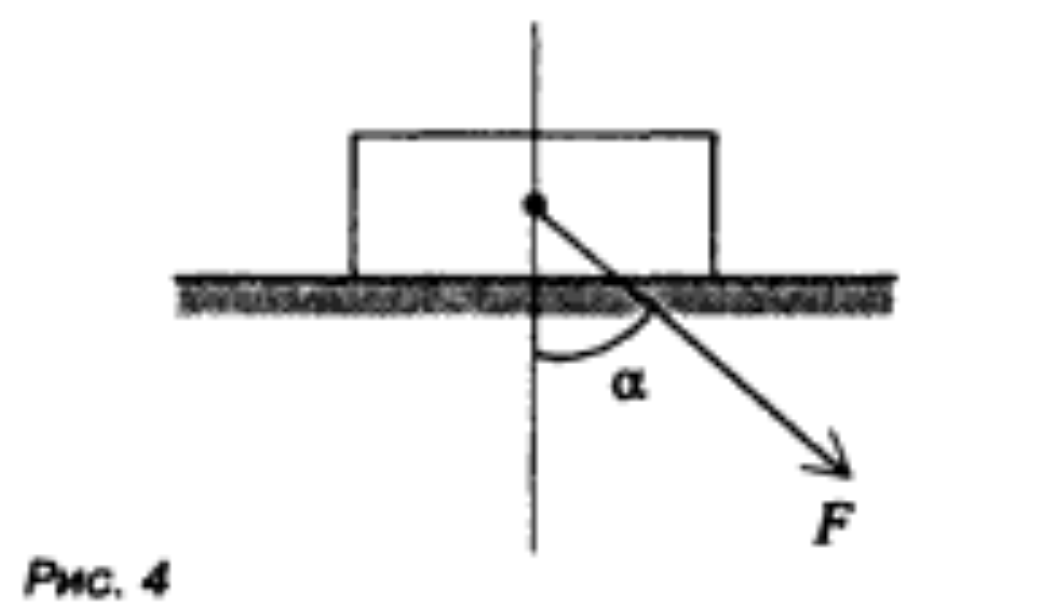
\includegraphics[scale=0.3]{images/image4.png}
\indent 3. Два шарика, радиусы которых отличаются в n = 5 раз, заряжены равными одноименными зарядами. Во сколько раз изменится сила взаимодействия между шариками, если их соединить проволкой?
\indent 4. Процессы, происходящие в цилинлре теплового двигателя с идеальным
\columnbreak
\noindent \small газом, изображены на диаграмме $p - V$ (рис.5). Известно, что $T_2 = 500 K, T_3 = 450 K, T_4 = 300 K$. Найдите на сколько градусов температура $T_1$ отличается от $T_3$.
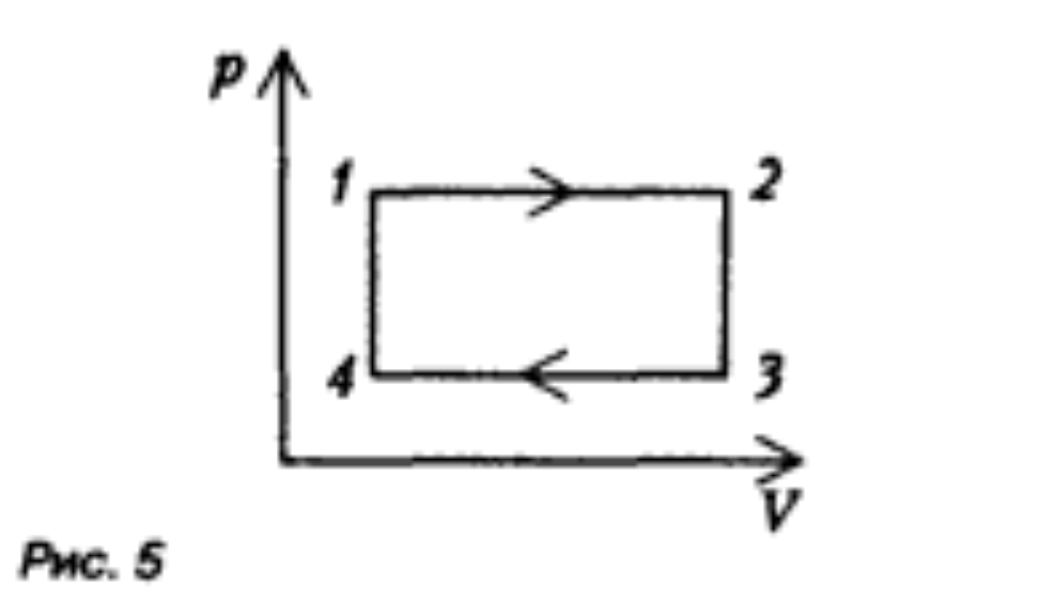
\includegraphics[scale=0.25]{images/image5.png}
\indent Внимание! Для учащихся 9 классов, поступающих в СУНЦ МГУ, в анкетных данных(на 1 странице работы) укажите профиль обучения: физико-математический, компьютерно-информационный, экономический, химический, биофизический. Поступающим на компьютерно-информационное, экономическое, химическое отделения необходимо решить дополнительный задачи по профилю.
\hline \hspace{5pt} \\
\noindent \normalsize Дополнительные задачи по информатике для поступающих на компьютерно-информационное отделение \\
\hspace{5pt} \hline 
\hspace{3pt} \\
\footnotesize \indent 1. Напишите программу на любом известном Вам языке программирования. Программа должна определять делится ли на 3 произвольное число, десятичная запись которого может содержать до N цифр $(N \le 1000)$. При этом нельзя использовать никаких операций деления(в том числе целочисленного деления и операцию взятие остатка от деления).
\indent 2. На единичной окружности задано N дуг $(N \le 1000)$. Начало и конец каждой дуги обозначаются целым числом градусов. Все дуги ориентированы по часовой стрелке, т.е. дуга $[300; 30]$ имеет «протяженность» 90 градусов, а дуга $[30; 300]$ - 270 градусов. Напишите программу, которая будет определять размер в градусах области пересечения всех дуг.
\hline \hspace{5pt} \\
\noindent \normalsize Дополнительные задачи по химии для поступающих на химическое отделение \\
\hspace{5pt} \hline
\hspace{3pt} \\
\footnotesize \indent 1. При нагревании 150г смеси бертолетовой соли с диоксидом марганца выделилось 33,6 л газа (н.у.). при растворении продуктов реакции в горячей воде осталось 3,0 г осадка. Определите состав (\%) твердых продуктов реакции.
\footnotesize \indent 2. При растворении 5,38 г кристаллогидрата сульфата цинка в 92 $cm^3$ воды получен раствор с массовой долей сульфата цинка 0,0331. Установите состав кристаллогидрата (Значение X).

\end{multicols*}

\begin{tabular}{|c|c|c|c|}
\hline & \multicolumn{2}{|c|}{ Затраты на единнцу продукции } & Объем ресурсов (M) \\
\cline { 2 - 3 } & шкаф & тумбочка & \\
\hline \begin{tabular}{c} 
Доска первого \\
типа (M)
\end{tabular} & 21 & 5 & 1340 \\
\hline \begin{tabular}{c} 
Доска второго \\
типа (м)
\end{tabular} & 10 & 7 & 1100\\
\hline Прибыль (руб.) & 2400 & 1000 & \\
\hline
\end{tabular}

\vspace{550pt}

\indent \large Источник: https://kvant.ras.ru/1994/06/novyj\_priem\_v\_sunc\_mgu\_i\_ngu.htm
